\documentclass[11pt]{article}

% Change "review" to "final" to generate the final (sometimes called camera-ready) version.
% Change to "preprint" to generate a non-anonymous version with page numbers.
\usepackage[review]{acl}

% Standard package includes
\usepackage{times}
\usepackage{latexsym}
\usepackage{booktabs}
% For proper rendering and hyphenation of words containing Latin characters (including in bib files)
\usepackage[T1]{fontenc}
% For Vietnamese characters
% \usepackage[T5]{fontenc}
% See https://www.latex-project.org/help/documentation/encguide.pdf for other character sets

% This assumes your files are encoded as UTF8
\usepackage[utf8]{inputenc}

% This is not strictly necessary, and may be commented out,
% but it will improve the layout of the manuscript,
% and will typically save some space.
\usepackage{microtype}

% This is also not strictly necessary, and may be commented out.
% However, it will improve the aesthetics of text in
% the typewriter font.
\usepackage{inconsolata}
\usepackage{xcolor}
%Including images in your LaTeX document requires adding
%additional package(s)
\usepackage{graphicx}
\usepackage{amsmath}
\usepackage{amsthm}
\usepackage{amssymb}
\theoremstyle{definition}          % 正文不斜体（适合 definition）
\newtheorem{definition}{Definition}[section]

\newcommand{\cmark}{\textcolor{green!60!black}{$\checkmark$}}
\newcommand{\xmark}{\textcolor{red}{$\times$}}

% If the title and author information does not fit in the area allocated, uncomment the following
%
%\setlength\titlebox{<dim>}
%
% and set <dim> to something 5cm or larger.

\title{Do Multiple Agents Predict Better? A Study of Information Splitting and Iterative Aggregation for Binary Market Forecasting}

% Author information can be set in various styles:
% For several authors from the same institution:
% \author{Author 1 \and ... \and Author n \\
%         Address line \\ ... \\ Address line}
% if the names do not fit well on one line use
%         Author 1 \\ {\bf Author 2} \\ ... \\ {\bf Author n} \\
% For authors from different institutions:
% \author{Author 1 \\ Address line \\  ... \\ Address line
%         \And  ... \And
%         Author n \\ Address line \\ ... \\ Address line}
% To start a separate ``row'' of authors use \AND, as in
% \author{Author 1 \\ Address line \\  ... \\ Address line
%         \AND
%         Author 2 \\ Address line \\ ... \\ Address line \And
%         Author 3 \\ Address line \\ ... \\ Address line}

\author{First Author \\
  Affiliation / Address line 1 \\
  Affiliation / Address line 2 \\
  Affiliation / Address line 3 \\
  \texttt{email@domain} \\\And
  Second Author \\
  Affiliation / Address line 1 \\
  Affiliation / Address line 2 \\
  Affiliation / Address line 3 \\
  \texttt{email@domain} \\}

%\author{
%  \textbf{First Author\textsuperscript{1}},
%  \textbf{Second Author\textsuperscript{1,2}},
%  \textbf{Third T. Author\textsuperscript{1}},
%  \textbf{Fourth Author\textsuperscript{1}},
%\\
%  \textbf{Fifth Author\textsuperscript{1,2}},
%  \textbf{Sixth Author\textsuperscript{1}},
%  \textbf{Seventh Author\textsuperscript{1}},
%  \textbf{Eighth Author \textsuperscript{1,2,3,4}},
%\\
%  \textbf{Ninth Author\textsuperscript{1}},
%  \textbf{Tenth Author\textsuperscript{1}},
%  \textbf{Eleventh E. Author\textsuperscript{1,2,3,4,5}},
%  \textbf{Twelfth Author\textsuperscript{1}},
%\\
%  \textbf{Thirteenth Author\textsuperscript{3}},
%  \textbf{Fourteenth F. Author\textsuperscript{2,4}},
%  \textbf{Fifteenth Author\textsuperscript{1}},
%  \textbf{Sixteenth Author\textsuperscript{1}},
%\\
%  \textbf{Seventeenth S. Author\textsuperscript{4,5}},
%  \textbf{Eighteenth Author\textsuperscript{3,4}},
%  \textbf{Nineteenth N. Author\textsuperscript{2,5}},
%  \textbf{Twentieth Author\textsuperscript{1}}
%\\
%\\
%  \textsuperscript{1}Affiliation 1,
%  \textsuperscript{2}Affiliation 2,
%  \textsuperscript{3}Affiliation 3,
%  \textsuperscript{4}Affiliation 4,
%  \textsuperscript{5}Affiliation 5
%\\
%  \small{
%    \textbf{Correspondence:} \href{mailto:email@domain}{email@domain}
%  }
%}

\begin{document}
\maketitle
\begin{abstract}
We propose a multi-agent LLM forecasting framework for binary prediction market questions.
To overcome the context limitations of single-agent approaches and enable effective
deliberation, we combine BM25-based evidence routing---which distributes query-relevant
documents across agents to create complementary private views---with Confidence-Weighted
(CW) aggregation, which weights agent forecasts by self-reported confidence.
On 497 Polymarket questions, our framework reduces the Brier score by 17.5\% and improves
accuracy by 6.6 percentage points over a single-agent baseline.
We further find that iterative deliberation yields no benefit without evidence diversity:
without BM25 routing, multi-round exchange leads to herding rather than genuine belief revision,
highlighting evidence routing as a critical design choice in multi-agent forecasting.
Our code is available at: \url{https://github.com/WinstonLiyt/PolymktSim}.
\end{abstract}

  % Large language models (LLMs) are increasingly applied to probabilistic
  % forecasting tasks, where a model must estimate the likelihood of real-world
  % events from retrieved textual evidence. Extending this paradigm to multi-agent
  % settings, where a panel of LLMs deliberates over shared predictions, is a
  % natural approach to improving forecast quality. However, existing multi-agent
  % pipelines suffer from a critical limitation: when agents are assigned
  % overlapping evidence, deliberation degenerates into reinforcement of the
  % majority view rather than genuine belief revision, a failure mode analogous
  % to herding in collective intelligence. This results in multi-round exchange
  % yielding little to no improvement over a single-agent baseline. We propose
  % a framework that addresses this by coupling relevance-aware evidence routing
  % with confidence-weighted aggregation. Specifically, we partition retrieved
  % documents using BM25 scores to construct complementary private views across
  % agents, ensuring information diversity as a prerequisite for effective
  % deliberation, and aggregate final-round forecasts by each agent's
  % self-reported confidence. On PolyGym, a dataset of 497 binary Polymarket
  % questions with temporally controlled evidence, our framework reduces Brier
  % score by 17.5\% and improves accuracy by 6.6 percentage points over a
  % single-agent RAG baseline. Ablation studies further confirm that evidence
  % routing is the load-bearing component: without it, iterative deliberation
  % provides no measurable benefit.

\section{Introduction}
\label{sec:intro}

Forecasting the outcomes of real-world events from textual evidence is a fundamental reasoning task with broad applications in decision support, risk assessment, and policy planning.
Prediction markets such as Polymarket provide a natural large-scale benchmark for this problem: questions resolve to binary outcomes with verifiable ground truth, and the associated evidence corpus is retrievable prior to resolution, enabling
controlled evaluation of evidence-grounded probabilistic reasoning.

Recent work has demonstrated that large language models (LLMs) can serve as effective zero-shot forecasters when provided with retrieved evidence~\citep{}.
A natural extension is the multi-agent setting, where a panel of LLM agents each
process a subset of available evidence and exchange predictions through iterative deliberation~\citep{}.
Such frameworks draw inspiration from human expert panels, where independently gathered knowledge is pooled and debated before a collective judgment is reached, and have shown promise in tasks requiring diverse reasoning perspectives~\citep{}.


Despite their appeal, existing multi-agent forecasting approaches face two key challenges.
First, \emph{evidence allocation} is typically handled by random splitting, which does not account for query relevance and may concentrate informative documents within a single agent's view while others receive peripheral evidence.
Second, and more fundamentally, multi-agent deliberation implicitly assumes that agents hold \emph{informationally diverse} views---yet when evidence partitions
overlap heavily, agents reach the same conclusions independently and iterative exchange degenerates into reinforcement rather than genuine belief revision, a failure mode analogous to herding in collective intelligence~\citep{}.
Existing aggregation methods treat agent forecasts as equally reliable signals, ignoring variation in the quality of each agent's private evidence.


We propose a multi-agent LLM forecasting framework grounded in the principle of \emph{information diversity maximization}.
To ensure agents hold complementary views, we introduce \textbf{BM25-based evidence routing}: documents are ranked by query relevance and distributed across agents via round-robin allocation, placing the most informative evidence in distinct private views and minimising inter-agent overlap.
Building on this diverse foundation, we show that iterative deliberation enables genuine belief revision across rounds.
To aggregate the resulting heterogeneous forecasts, we propose \textbf{Confidence-Weighted (CW) aggregation}, which treats self-reported agent confidence as a proxy for evidence quality and up-weights agents whose private evidence supports a stronger prior.

We evaluate our framework on 497 binary forecasting questions from Polymarket,
spanning domains including cryptocurrency, sports, and politics.
Our main findings are:
\begin{itemize}
  \item CW + BM25 with iterative deliberation reduces Brier score by \textbf{17.5\%}
    and improves accuracy by \textbf{6.6 percentage points} over a single-agent baseline.
  \item Iterative deliberation is only effective when agents hold genuinely diverse views:
    without BM25 routing, deliberation provides no measurable benefit, consistent with
    the herding phenomenon in collective intelligence.
  \item Confidence-weighted aggregation improves decision accuracy over the arithmetic
    mean, demonstrating that agent self-assessments carry predictive signal beyond the
    probability estimate itself.
\end{itemize}


\section{Related Work}

\textbf{LLM-based Forecasting Pipelines.}
Early work on LLM forecasting established a large gap between machine and human performance.
\citet{zou2022forecasting} introduce Autocast, a benchmark of thousands of real-world questions drawn from Metaculus and Good Judgment Open, finding that the best language models achieve only~38\% accuracy compared to~82\% for human aggregates.
\citet{schoenegger2023large} further enroll GPT-4 in a live Metaculus tournament, finding its unaugmented predictions do not significantly outperform a naive 50\% baseline.
These results motivate the use of retrieval-augmented generation (RAG)~\citep{lewis2020retrieval,guu2020retrieval} to ground LLM outputs in external evidence.
\citet{yanautocast++} demonstrate that zero-shot re-ranking and summarization of retrieved news articles improves LLM forecasting accuracy by up to 48\% on Autocast, while \citet{piryani2025s} show that news articles are the single most impactful context type, significantly outperforming background text or few-shot examples.
Building on these findings, \citet{halawi2024approaching} present a full pipeline that automates retrieval, summarization, and aggregation of LLM probability estimates for binary events, achieving near-human-level performance on Polymarket and Metaculus questions.
More recently, \citet{turtel2025llms} apply outcome-based fine-tuning on 12,100 resolved Polymarket questions, while \citet{chandakscaling} train an open-source 8B model via reinforcement learning that matches proprietary LLMs on prediction market benchmarks.

On the aggregation side, \citet{schoenegger2024wisdom} find that ensembling 12 diverse LLMs produces forecasts statistically indistinguishable from a crowd of 925 human forecasters, establishing a ``wisdom of the silicon crowd'' effect parallel to human crowd wisdom.
Aggregating outputs from multiple LLMs has also been studied in broader reasoning contexts: \citet{wangself} show that sampling diverse chain-of-thought paths and selecting by majority vote improves reasoning accuracy, while \citet{wangmixture} propose Mixture-of-Agents (MoA), a layered architecture where later agents condition on all earlier outputs, achieving state-of-the-art performance on general benchmarks.
\citet{chen2024reconcile} further demonstrate that a round-table conference of diverse LLMs with confidence-weighted voting outperforms both single-agent and homogeneous multi-agent baselines across seven reasoning benchmarks.

Evaluation methodology in this domain requires careful contamination control.
ForecastBench~\citep{karger2024forecastbench} and FutureX~\citep{zeng2025futurex} provide continuously updated benchmarks sourcing questions from Polymarket and other platforms, where resolutions strictly postdate any training data.
\citet{paleka2025pitfalls} identify systematic pitfalls including temporal leakage via web search and piggybacking on existing human forecasts, motivating strict timestamp-based evidence cutoffs.
For uncertainty quantification, \citet{lin2022teaching} show that LLMs can be fine-tuned to express calibrated verbalized probabilities, and \citet{tian2023just} demonstrate that verbalized confidence scores are typically better calibrated than token-level log-probabilities for RLHF-tuned models.

Despite these advances, existing pipelines treat forecasting as a single-agent, single-pass process. Whether structured multi-agent interaction over \emph{split} evidence improves probabilistic predictions on binary prediction market questions remains an open question.

\paragraph{Iterative Forecast Aggregation}

\paragraph{Probabilistic aggregation.}
The linear opinion pool~\citep{9ca5e582-1e4c-323f-9ab1-c62032d22e48}, which computes a weighted average of individual probability forecasts, is the most widely used aggregation method.
However, \citet{10.1111/j.1467-9868.2009.00726.x} show that it generally produces underconfident and miscalibrated aggregates when individual forecasts differ, as convex combination compresses predictions toward the base rate.
\citet{SATOPAA2014344} address this limitation by proposing a logit-space aggregation with an extremizing factor, validated on IARPA geopolitical forecasting tournaments.
The theoretical basis for extremizing is formalized by \citet{abernethy2014information}, who show that the optimal degree of extremizing depends on the level of information overlap among forecasters: lower overlap calls for stronger extremization.
\citet{10.1214/ss/1177013825} provide an axiomatic treatment of opinion pooling, proving that the logarithmic opinion pool uniquely satisfies external Bayesianity.


\paragraph{Iterative interaction and social dynamics.}
\citet{612bb50a-4bdd-3a32-b6eb-7837600cc9c4} models iterative opinion updating as repeated weighted averaging over a social network, proving convergence to a consensus determined by the eigenvector centrality of the influence graph. The Delphi method~\citep{DALKEY1969408} instantiates a similar process in human expert elicitation, where participants revise estimates across structured rounds after receiving aggregate feedback, empirically reducing inter-rater variance. \citet{LONKANI2026106120} demonstrate in large-scale forecasting tournaments that team collaboration and algorithmic aggregation jointly improve accuracy beyond individual performance. On the other hand, \citet{Lorenz2011HowSI} show experimentally that social influence can collapse forecast diversity without improving accuracy, producing collective overconfidence. \citet{bikhchandani1992theory} formalize informational cascades, demonstrating that rational agents may discard private signals entirely once public opinion reaches a tipping point. Taken together, these works reveal a fundamental tension: iterative interaction can either extract complementary private information or induce herding, yet this tradeoff has not been empirically examined in LLM-based probabilistic forecasting.

\section{Dataset Construction}
We construct \textsc{PolyGym} from a large-scale Polymarket dataset\footnote{\url{https://www.kaggle.com/datasets/ismetsemedov/polymarket-prediction-markets}} consisting of approximately 40k events and 100k associated prediction markets.
Each event represents a high-level topic, while individual markets correspond to specific binary forecasting questions linked via event identifiers.

\paragraph{Topic normalization and sampling.}
To obtain a coherent topic structure, we first assign events to canonical domains using metadata fields (e.g., titles, descriptions, and tags), and propagate these labels to their associated markets.
We then construct the dataset via \emph{popularity-weighted sampling}, allocating quotas across topics proportional to market activity (e.g., volume and liquidity).
This ensures realistic coverage of high-impact domains while maintaining diversity.
The final dataset contains 500 markets spanning multiple domains.

\paragraph{Evidence construction.}
For each market, we build an evidence corpus through tavily search API\footnote{\url{https://www.tavily.com/}}.
We generate multiple queries based on the question and event context, retrieve candidate documents, and enforce a strict temporal cutoff such that all evidence precedes the market resolution time.
Retrieved documents are deduplicated, ranked, and truncated to a fixed size to ensure consistency across instances.

\paragraph{Final dataset.}
Each instance consists of a forecasting question, its resolution time, a time-aligned evidence set, and a ground-truth outcome.
This construction yields a high-quality and reproducible benchmark for evidence-based forecasting.
Detailed information is provided in Appendix~.

\begin{table*}[t]
\centering
\small
\begin{tabular}{lccccccc}
\toprule
\textbf{Setup} & \textbf{Live} & \textbf{Static} & \textbf{Reproducible} & \textbf{Time Control} & \textbf{Fixed Evidence} & \textbf{Realistic} & \textbf{Agent Study} \\
\midrule
ForecastBench~\citep{karger2024forecastbench} & \cmark & \xmark & \xmark & \cmark & \xmark & \cmark & \xmark \\
FutureX~\citep{zeng2025futurex} & \cmark & \xmark & \xmark & \cmark & \xmark & \cmark & \xmark \\
PolyBench~\citep{cheng2026polybench} & \cmark & \xmark & \xmark & \cmark & \xmark & \cmark & \xmark \\
Prediction Arena~\citep{zhang2026predictionarena} & \cmark & \xmark & \xmark & \cmark & \xmark & \cmark & \cmark \\
Zou et al.~\citep{zou2022forecasting} & \xmark & \cmark & \xmark & \xmark & \xmark & \xmark & \xmark \\
Halawi et al.~\citep{halawi2024approaching} & \xmark & \cmark & \xmark & \xmark & \xmark & \xmark & \xmark \\
\midrule
\textbf{PolyGym (Ours)} & \xmark & \cmark & \cmark & \cmark & \cmark & \cmark & \cmark \\
\bottomrule
\end{tabular}
\caption{
Comparison of forecasting evaluation setups.
Existing approaches fall into two categories: (1) live benchmarks with high realism but limited reproducibility (ForecastBench, FutureX, PolyBench, Prediction Arena), and (2) static setups lacking strict temporal and evidence control (Zou et al., Halawi et al.).
PolyGym uniquely provides a controlled, reproducible environment with fixed evidence and strict temporal filtering, enabling principled evaluation of reasoning and multi-agent aggregation.
}
\end{table*}

\section{Methodology}
\subsection{Problem Definition}
Let $q$ denote a natural-language binary forecasting question with associated resolution
date $\tau \in \mathcal{T}$ and ground-truth outcome $y \in \{0,1\}$, where $y=1$ denotes
the event resolving \textsc{Yes}.
Each question is accompanied by a retrieved evidence corpus
$\mathcal{E} = \{e_1, \dots, e_n\}$, where each item $e_i = (d_i, t_i, c_i)$ consists of
a document identifier $d_i$, a publication timestamp $t_i$, and textual content $c_i$.

\begin{definition}[Binary Forecasting]
Given a question $q$, resolution date $\tau$, and evidence corpus $\mathcal{E}$,
a \emph{forecast} is a probability estimate $\hat{p} \in [0,1]$ for the event $y=1$.
A dataset is a collection $\mathcal{Q} = \{(q_k, \tau_k, \mathcal{E}_k, y_k)\}_{k=1}^{N}$
of forecasting instances with known outcomes.
\end{definition}


\subsection{Overview}

% Figure~\ref{fig:overview} illustrates the end-to-end pipeline.
% Given a binary forecasting question $q$ and its associated evidence corpus $\mathcal{E}$,
% our framework proceeds in three stages.

% \textbf{(1) Evidence Routing.}
% The corpus is split into a shared public portion $\mathcal{E}^{\mathrm{pub}}$,
% visible to all agents, and $J$ private portions $\{\mathcal{E}_j^{\mathrm{priv}}\}$
% allocated via BM25-based relevance ranking.
% Unlike random splitting, relevance-aware routing ensures that the most
% informative documents are distributed across distinct agent views,
% promoting \emph{informational diversity} rather than redundancy.

% \textbf{(2) Multi-Agent Deliberation.}
% Each agent $A_j$ receives its private view $\mathcal{E}_j$ and independently
% produces an initial forecast.
% Under the iterative deliberation protocol, agents observe a summary of
% all prior-round predictions and revise their beliefs over $R$ rounds,
% enabling \emph{sequential belief updating} akin to a structured discussion.

% \textbf{(3) Confidence-Weighted Aggregation.}
% Final-round forecasts are combined via CW aggregation~\eqref{eq:cw},
% which up-weights agents that express higher self-reported confidence,
% yielding a single calibrated probability estimate $\hat{p}_{\mathrm{CW}}$.

% The three stages are designed to address distinct failure modes of single-agent
% forecasting: evidence routing mitigates context truncation and promotes diversity;
% iterative deliberation reduces overconfidence from limited private information;
% and confidence-weighted aggregation discounts uncertain agents whose private
% evidence does not support a strong prior.

As illustrated in Figure~\ref{fig:overview}, our framework comprises three stages:
(1)~BM25-based relevance routing partitions the evidence corpus into diverse agent-specific views;
(2)~a panel of $J$ LLM agents deliberates over $R$ rounds, with each round's predictions
broadcast as a shared history to support belief revision;
(3)~final-round forecasts are aggregated via confidence-weighted pooling into a single
probability estimate.

\subsection{Evidence Partition and BM25 Routing}

We consider a panel of $J$ LLM-based agents $\{A_1, \dots, A_J\}$.
Let $\rho \in [0,1]$ be the \emph{public ratio}.
The corpus $\mathcal{E}$ is partitioned into a shared public subset $\mathcal{E}^{\mathrm{pub}}$
and $J$ disjoint private subsets $\{\mathcal{E}_j^{\mathrm{priv}}\}_{j=1}^{J}$:
\begin{equation}
  \mathcal{E} \;=\; \mathcal{E}^{\mathrm{pub}} \;\cup\; \bigsqcup_{j=1}^{J} \mathcal{E}_j^{\mathrm{priv}},
  \qquad
  |\mathcal{E}^{\mathrm{pub}}| \;=\; \lfloor \rho \cdot |\mathcal{E}| \rfloor.
  \label{eq:partition}
\end{equation}
Each agent $A_j$ observes the \emph{private view}
$\mathcal{E}_j = \mathcal{E}^{\mathrm{pub}} \cup \mathcal{E}_j^{\mathrm{priv}}$.

To maximise information diversity across agents, private subsets are allocated via
relevance-aware routing rather than random splitting.
Each document $e_i \in \mathcal{E} \setminus \mathcal{E}^{\mathrm{pub}}$ receives a BM25
relevance score $s_i = \mathrm{BM25}(e_i, q)$.
Documents are ranked by $s_i$ in descending order and assigned to agents
in a round-robin fashion, so that the most query-relevant evidence is
spread across distinct private views.

\subsection{Multi-Agent Deliberation}

\paragraph{Individual Forecast.}
At round $r$, agent $A_j$ produces a structured forecast
$f_j^{(r)} = \bigl(p_j^{(r)},\, \ell_j^{(r)},\, u_j^{(r)}\bigr)$,
where $p_j^{(r)} \in [0,1]$ is a probability estimate,
$\ell_j^{(r)} \in \{\textsc{Yes},\textsc{No}\}$ is a categorical label,
and $u_j^{(r)} \in \{0,1,2\}$ encodes self-reported confidence
(low / medium / high).
The agent conditions on its private view $\mathcal{E}_j$
and a history summary $h^{(r-1)}$ of prior-round forecasts ($h^{(0)} = \varnothing$):
\begin{equation}
  f_j^{(r)} \;\sim\; \mathrm{LLM}\!\left(q,\; \mathcal{E}_j,\; h^{(r-1)}\right).
  \label{eq:agent}
\end{equation}

\paragraph{Deliberation Protocols.}
We consider two interaction protocols: (i) \textbf{Independent Forecasting.} Each agent forecasts once ($R=1$) without observing others' predictions ($h^{(0)} = \varnothing$). Agents reason solely from their private view. (ii) \textbf{Iterative Deliberation.} Agents forecast over $R > 1$ rounds. After each round $r < R$, all individual forecasts are summarised into $h^{(r)} = \mathrm{Summarise}\!\bigl(\{f_j^{(r)}\}_{j=1}^{J}\bigr)$ and broadcast to all agents, enabling belief revision in subsequent rounds.

\subsection{Confidence-Weighted Aggregation}

Given the final-round forecasts $\{f_j\}_{j=1}^{J}$, a \emph{forecast aggregator}
$\mathcal{A}$ combines them into a single prediction $\hat{p} = \mathcal{A}(f_1, \dots, f_J)$.

We propose \emph{Confidence-Weighted (CW) aggregation}, which scales each agent's
contribution by its self-reported confidence.
Define the confidence weight $w_j = \phi(u_j)$, where
$\phi : \{0,1,2\} \to \mathbb{R}_{>0}$ is a monotone mapping
(concretely, $\phi(u) = u + 1$, yielding weights $1, 2, 3$).
The aggregated forecast is:
\begin{equation}
  \hat{p}_{\mathrm{CW}} \;=\; \frac{\displaystyle\sum_{j=1}^{J} w_j \, p_j}
                                    {\displaystyle\sum_{j=1}^{J} w_j}.
  \label{eq:cw}
\end{equation}
When all agents report equal confidence, \eqref{eq:cw} reduces to the arithmetic mean.
Agents expressing higher confidence receive greater influence in the collective prediction,
reflecting the intuition that a well-evidenced agent should not be equally weighted with
an uncertain one.

\section{Experiment}
\subsection{Experiment Setup}
\paragraph{Datasets.}
We evaluate on a collection of 500 binary forecasting questions sourced from Polymarket,\footnote{\url{https://polymarket.com}} a real-money prediction market platform.
Each question is paired with up to 30 retrieved evidence documents and a known binary outcome $y \in \{0,1\}$.
Questions span multiple domains, with Crypto (60\%), Sports (22\%), Science \& Technology (9\%), Politics (7\%), and Business (6\%) as the principal categories.
For each question, evidence documents were retrieved prior to the resolution date $\tau$ and truncated to at most 500 characters per document to control context length.
After filtering questions with unresolved outcomes, 497 questions are used for evaluation.
Details of the curation of the dataset are in Appendix \ref{sec:dataset}.

\paragraph{Baselines.}
xxx

\paragraph{Metrics.}
We report two complementary metrics.
The \emph{Brier score} $\mathrm{BS} = \frac{1}{N}\sum_{k=1}^{N}(\hat{p}_k - y_k)^2$ measures probabilistic calibration.
\emph{Accuracy} reports the fraction of questions for which the predicted label $\mathbf{1}[\hat{p} \geq 0.5]$ matches the ground-truth outcome $y$.

\paragraph{Implementation Details.}
All agents are instantiated from \texttt{gpt-5.4-mini} accessed via the OpenRouter API.
We use $J = 3$ agents and $R = 2$ deliberation rounds.
The public evidence ratio is set to $\rho = 0.5$, so half of the evidence corpus is shared across all agents and the remainder is split privately.
Agent responses are sampled at temperature $T = 0.7$.
All experiments use a fixed random seed of 42.

\subsection{Main Results}



Table~\ref{tab:main} reports Brier score and accuracy for all methods under both
the independent forecasting and iterative deliberation protocols.

\begin{table}[t]
\centering
\caption{Results on the Polymarket binary forecasting benchmark ($N=497$).
  \textbf{Bold} denotes the best result per column; \underline{underline} the second best.
  ``Indep.'' refers to independent forecasting ($R=1$); ``Iter.'' to iterative deliberation ($R=2$).}
\label{tab:main}

\resizebox{\columnwidth}{!}{
\begin{tabular}{lcccc}
\toprule
 & \multicolumn{2}{c}{\textbf{Independent}} & \multicolumn{2}{c}{\textbf{Iterative}} \\
\cmidrule(lr){2-3}\cmidrule(lr){4-5}
\textbf{Method} & Brier$\downarrow$ & Acc$\uparrow$ & Brier$\downarrow$ & Acc$\uparrow$ \\
\midrule
Single-Agent        & 0.2116 & 71.6\% & — & — \\
Mean                & 0.1941 & 71.0\% & 0.1944 & 71.2\% \\
Mean + BM25         & \underline{0.1897} & 71.0\% & \underline{0.1712} & \underline{77.8\%} \\
Mean (All info) & 0.2120 & 70.0\% & 0.2028 & 70.4\% \\
CW                  & 0.2188 & 70.2\% & 0.1865 & 76.2\% \\
CW + BM25 (ours)    & 0.2051 & \textbf{73.4\%} & \textbf{0.1746} & \textbf{78.2\%} \\
\bottomrule
\end{tabular}
}
\end{table}
\paragraph{Overall performance.}
CW + BM25 with iterative deliberation achieves the best accuracy (78.2\%) and the
second-best Brier score (0.1746), reducing the Brier score relative to the single-agent
baseline by 17.5\% and improving accuracy by 6.6 percentage points.
Mean + BM25 yields the lowest Brier score (0.1712) but slightly lower accuracy (77.8\%),
suggesting that confidence-weighted aggregation provides better-calibrated decisions at
the classification threshold while mean aggregation is marginally superior for probabilistic
calibration.

\paragraph{Effect of iterative deliberation.}
Iterative deliberation substantially benefits methods with BM25 routing:
CW + BM25 improves from 0.2051 to 0.1746 in Brier score (−14.9\%) and from 73.4\%
to 78.2\% in accuracy (+4.8 pp) when agents deliberate over two rounds.
In contrast, mean aggregation without BM25 shows virtually no improvement from
independent to iterative forecasting (0.1941 vs.\ 0.1944), indicating that deliberation
is only effective when agents hold genuinely diverse views.
Without evidence diversity, iterative rounds lead agents to converge on a shared belief
without introducing new information, a phenomenon consistent with group herding in
the collective intelligence literature.

\paragraph{Effect of BM25 evidence routing.}
BM25 routing consistently benefits both aggregators.
For confidence-weighted aggregation, replacing random splitting with BM25 routing
reduces the Brier score from 0.1865 to 0.1746 under iterative deliberation (−6.4\%),
while also improving accuracy from 76.2\% to 78.2\%.
The gain is even more pronounced for mean aggregation (0.1944 → 0.1712, −11.9\%).
These results confirm that routing evidence by query relevance creates more
informationally complementary private views, enabling more effective collective reasoning.

\paragraph{Effect of confidence-weighted aggregation.}
Under independent forecasting, CW + BM25 achieves higher accuracy (73.4\%) than
Mean + BM25 (71.0\%), demonstrating that self-reported agent confidence is a useful
signal for weighting predictions.
Under iterative deliberation, CW + BM25 retains a 0.4 pp accuracy advantage over
Mean + BM25, suggesting that agents' confidence estimates remain informative even after
multi-round belief updating.

\subsection{Prediction extremity as a proxy for evidence quality.}
To assess whether prediction extremity is a reliable signal of forecast quality,
we collect all 1,491 individual agent predictions from the CW + BM25 independent
forecasting setting, compute the extremity $|p - 0.5|$ for each, and sort them
into four equal-sized quartiles (Q1: least extreme, Q4: most extreme).
We then compute accuracy and Brier score within each quartile independently.
Figure~\ref{fig:extremity} stratifies individual agent forecasts by prediction
extremity $|p - 0.5|$ into four quartiles and reports accuracy and Brier score for
each group.
Accuracy increases monotonically from 48.1\% in the most uncertain quartile (Q1,
where agents assign probabilities close to 0.5) to 92.3\% in the most confident
quartile (Q4), while Brier score falls from 0.279 to 0.075.
This strong monotonic relationship validates the design of CW aggregation:
agents that produce more extreme probability estimates are substantially more
accurate, and up-weighting them via $w_j = |\mathrm{logit}(p_j)|$ concentrates
influence in the agents whose private evidence most strongly supports a clear outcome.

\begin{figure}[t]
  \centering
  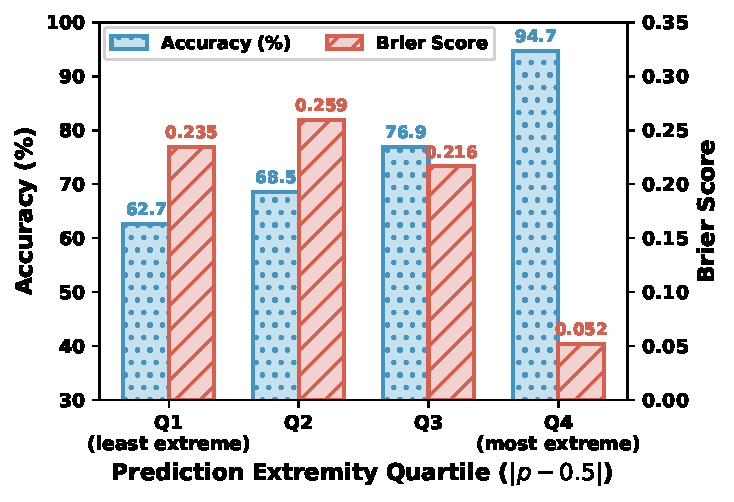
\includegraphics[width=\linewidth]{fig1_extremity_accuracy.pdf}
  \caption{Accuracy and Brier score by agent prediction extremity quartile
    ($|p - 0.5|$), computed over all CW + BM25 agent forecasts ($N=1{,}491$).
    More extreme predictions correlate strongly with higher accuracy,
    validating the confidence-weighted aggregation design.}
  \label{fig:extremity}
\end{figure}

\subsection{BM25 routing suppresses herding.}

To quantify the degree of herding under different routing strategies, we measure
the mean inter-agent prediction variance at Round 1 (before belief exchange) and
Round 2 (after one round of deliberation) for three settings: All Info
($\rho = 1.0$, all agents observe the full corpus), Random Split ($\rho = 0.5$,
random allocation), and BM25 Split ($\rho = 0.5$, relevance-ranked allocation).
For each question, we compute the variance of the three agents' $p_{\mathrm{yes}}$
values at each round, and report the mean across all 497 questions.
Figure~\ref{fig:variance} compares the mean inter-agent prediction variance before
and after deliberation across three evidence routing settings.
Under \emph{All Info} (all agents see the full corpus), agents begin with low
initial variance and converge further after one round of exchange (89\% reduction),
exhibiting near-complete herding.
Under \emph{Random Split}, agents start with higher initial variance but converge
even more aggressively (91\% reduction), indicating that diverse initial predictions
alone do not prevent herding when agents lack access to complementary evidence.
Under \emph{BM25 Split}, deliberation reduces variance by only 71\%, preserving
substantially more inter-agent diversity.
This retained diversity reflects genuine belief revision---agents holding
complementary evidence continue to weight distinct aspects of the problem even after
observing others' predictions---rather than blind convergence toward the group mean.

\begin{figure}[t]
  \centering
  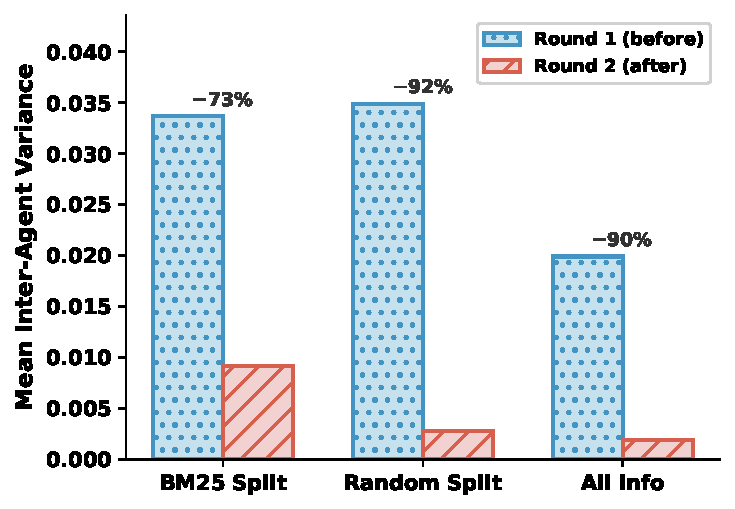
\includegraphics[width=\linewidth]{fig2_agent_variance.pdf}
  \caption{Mean inter-agent prediction variance before (Round 1) and after
    (Round 2) deliberation for three evidence routing settings.
    All Info and Random Split exhibit aggressive herding (89--91\% variance
    reduction), while BM25 Split retains substantially more diversity (71\%
    reduction), enabling genuine belief revision.}
  \label{fig:variance}
\end{figure}



\subsection{API Backends}

\resizebox{\columnwidth}{!}{
\begin{tabular}{lcccc}
\toprule
\textbf{Model} 
& \multicolumn{2}{c}{\textbf{Independent}} 
& \multicolumn{2}{c}{\textbf{Iterative}} \\
\cmidrule(lr){2-3}\cmidrule(lr){4-5}
& Brier$\downarrow$ & Acc$\uparrow$ 
& Brier$\downarrow$ & Acc$\uparrow$ \\
\midrule

GPT-5.4-mini        & 0.2051 & 73.4\% & 0.1746 & 78.2\% \\
gemini-3-flash-preview & 0.1766 & 81.1\% & 0.1760 & 81.5\% \\
glm-5 & & & &  \\
deepseek-v3.2 & 0.1837 & 76.1\% & 0.1611 & 80.5\% \\
\bottomrule
\end{tabular}
}


\section{Conclusion}
\label{sec:conclusion}

We presented a multi-agent LLM forecasting framework for binary prediction market
questions that combines BM25-based evidence routing with confidence-weighted aggregation
and iterative deliberation.
On a benchmark of 497 Polymarket questions, our method reduces the Brier score by
17.5\% and improves accuracy by 6.6 percentage points over a single-agent baseline.

A key finding is that evidence diversity is a prerequisite for effective deliberation.
Without BM25 routing, iterative rounds of belief exchange provide no benefit over
independent forecasting, as agents with overlapping evidence converge without
introducing new information.
Once routing creates genuinely complementary private views, multi-round deliberation
substantially improves calibration and accuracy.
Confidence-weighted aggregation further benefits decision accuracy by leveraging
agents' self-assessments as a proxy for evidence quality.

\paragraph{Limitations.}
Self-reported confidence is an imperfect proxy for epistemic reliability: agents may
be systematically overconfident or express uniform confidence regardless of evidence
quality.
Our evaluation is currently limited to one model family (\texttt{gpt-5.4-mini}),
and results may differ with larger or instruction-tuned models.
Evidence documents are truncated to 500 characters, which may discard relevant content
in longer articles.

\paragraph{Future work.}
An important direction is replacing self-reported confidence with calibrated uncertainty
estimates derived from logit distributions or ensemble disagreement.
Dynamic routing strategies that adapt evidence allocation based on emerging agent
disagreement across rounds represent another promising extension.
Scaling to larger agent panels and more deliberation rounds, with explicit mechanisms
to detect and mitigate herding, would further strengthen the framework.


% \section*{Limitations}

% This document does not cover the content requirements for ACL or any
% other specific venue.  Check the author instructions for
% information on
% maximum page lengths, the required ``Limitations'' section,
% and so on.

\section*{Acknowledgments}

This document has been adapted
by Steven Bethard, Ryan Cotterell and Rui Yan
from the instructions for earlier ACL and NAACL proceedings, including those for
ACL 2019 by Douwe Kiela and Ivan Vuli\'{c},
NAACL 2019 by Stephanie Lukin and Alla Roskovskaya,
ACL 2018 by Shay Cohen, Kevin Gimpel, and Wei Lu,
NAACL 2018 by Margaret Mitchell and Stephanie Lukin,
Bib\TeX{} suggestions for (NA)ACL 2017/2018 from Jason Eisner,
ACL 2017 by Dan Gildea and Min-Yen Kan,
NAACL 2017 by Margaret Mitchell,
ACL 2012 by Maggie Li and Michael White,
ACL 2010 by Jing-Shin Chang and Philipp Koehn,
ACL 2008 by Johanna D. Moore, Simone Teufel, James Allan, and Sadaoki Furui,
ACL 2005 by Hwee Tou Ng and Kemal Oflazer,
ACL 2002 by Eugene Charniak and Dekang Lin,
and earlier ACL and EACL formats written by several people, including
John Chen, Henry S. Thompson and Donald Walker.
Additional elements were taken from the formatting instructions of the \emph{International Joint Conference on Artificial Intelligence} and the \emph{Conference on Computer Vision and Pattern Recognition}.

% Bibliography entries for the entire Anthology, followed by custom entries
%\bibliography{anthology,custom}
% Custom bibliography entries only
\bibliography{custom}

\appendix


\section{Appendix: PolyGym — Rationale for a Standardized Offline Benchmark}
\label{sec:dataset}
\subsection*{Design Philosophy and Dataset Construction}
PolyGym is founded on the premise that for news and current events, the foundational information retrieved via search is largely consistent and commodified. Although severe information asymmetry can decisively impact specific prediction markets, such instances are exceptional outliers. Our primary objective is to elevate decision-making capabilities across general predictive tasks. Therefore, the true bottleneck in agentic AI lies not in uncovering exclusive data, but in making calibrated, rational decisions based on a standardized set of finite, high-quality evidence. To address this, we provide a high-quality, static environment derived from Polymarket. PolyGym isolates the reasoning component by offering a controlled subset of 500 questions curated through popularity-weighted sampling. This ensures the benchmark focuses on high-stakes, real-world events across politics, finance, and technology with maximum signal. Each query is paired with pre-fetched evidence retrieved via tavily search API\footnote{\url{https://www.tavily.com/}}, enabling a pure evaluation of an agent's ability to reconcile conflicting data without the interference of fluctuating search rankings.

\subsection*{Competitive Advantages and Seamless Deployment}
The PolyGym framework offers several advantages over "in-the-wild" testing environments. By fixing the information ceiling, it provides a stable environment for reproducible iteration, allowing developers to precisely measure how architectural changes affect decision quality without the noise of API volatility. Furthermore, PolyGym enforces structural rigor through a strict binary format (Yes/No questions), enabling objective scoring via accuracy and Brier calibration. To prevent look-ahead bias, we utilize a time-restricted search limit that ensures evidence is retrieved only from periods prior to an event’s resolution. Moreover, by employing importance sampling, PolyGym curates a highly representative dataset of high-stakes events. This systematically avoids the temporal bias inherent in live benchmarks, where evaluating a model's performance over an arbitrary single week can be heavily skewed by the anomalous news cycle of that specific period. Finally, PolyGym allows developers to iterate rapidly in a cost-effective static environment and then migrate to real-time testing benchmarks like FutureX by simply swapping the static evidence loader for a live search API.
\end{document}
